\documentclass{article}
\usepackage[utf8]{inputenc}
\usepackage{vntex}
\usepackage{hyperref}
\usepackage{float}
\usepackage{graphicx}
\usepackage{amsmath}
\usepackage{amssymb}
\title{Project: Job correlate with major choosing in VietNam}
\author{Huynh Phuong Nhu}
\date{Octorber 2021}
\begin{document}

\maketitle

\section{Inspiration}
\subsection{Introduction}
When talking about job, it all boils down to the core problem: What skill set and techniques give us the kind of job we want? We both know to each other that many consider a good job to be a well-paid one which also fit your color. That's why many adolescent seek for a university major that can better their life, this trend can clearly be seen in VietNam. As for a sister, whose brother is going to end his life in high school pretty soon, I want to make a prediction or a story-telling project to my brother because he is not the one who have vision for his future job and either the ability to do something major in this world. \\
Talking about major, there is some trend in the world of parent-picking one, searching for the term "Ngành học" which means "majors" on Google Trend on the 27th of September 2021, apart from queries about universities, scores to get into these, and which departments people can get in with kind of combination tests in the top 25 queries of 2021, we see some shows up on top: "Economics", "Marketing", "Business Adminstration" and "Information Techonology". Also the trend of looking for major peaked at week 31 when all the students recieve their national graduation test score have given us a glimpse as for one of the elements they choose major based on: score.\\

\begin{figure}[H]
	\begin{center}
		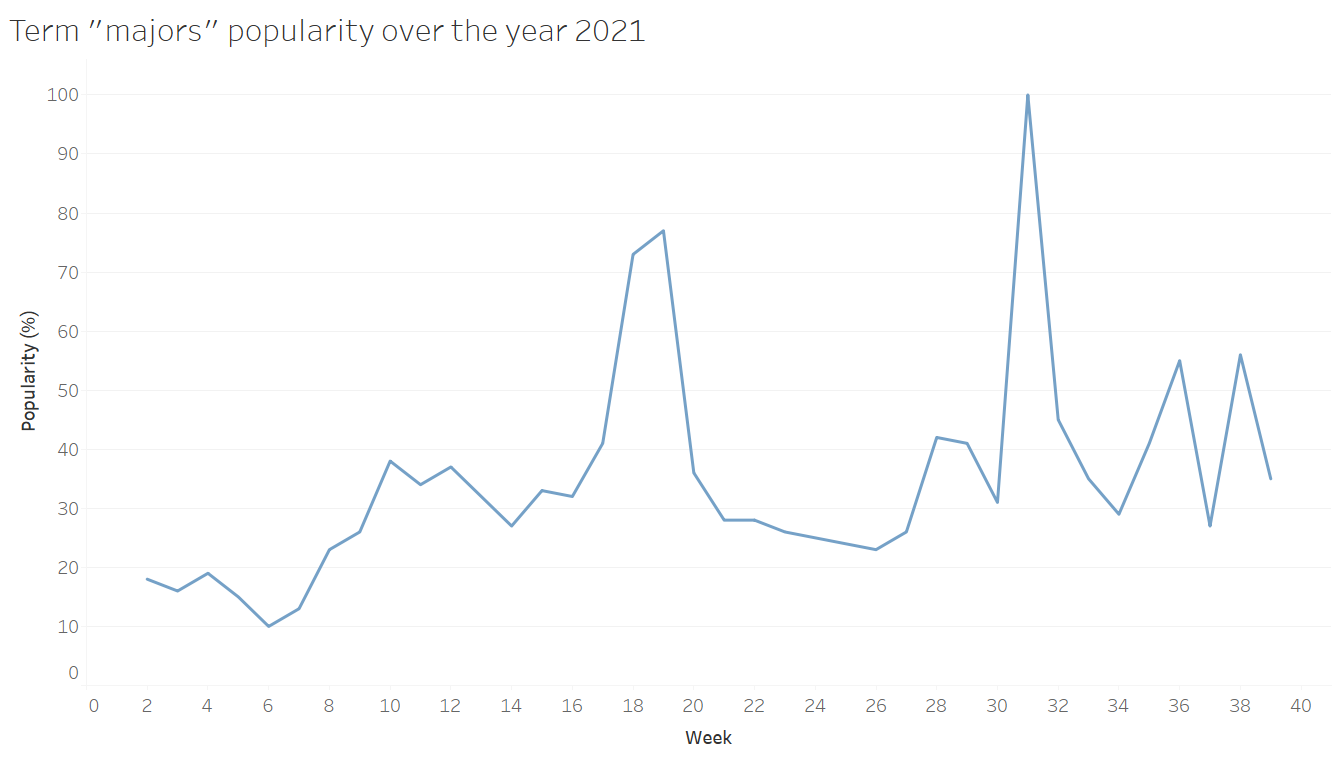
\includegraphics[scale=0.6]{Term-Popularity.png}
	\end{center}
	\caption{The term "Ngành học" popularity over the year 2021}
\end{figure}

We all know that the majority of undergraduates does not have work until their trainee lives at junior or senior years or even graduated from school. It will aproximately take them around 3,5 to 4 years to be able to reach the qualification of graduation. I want to see whether the occupation that you are targeted the day you enter your university still posisble for you to get in the year of your graduation and how long will one major trends set off and disappear.

So, we will need some data from a job site, data about education. I am planning to take information for the last 10 years.



\end{document}